\documentclass[12pt]{article}
\usepackage{amsmath}
\usepackage{amssymb}
\usepackage{amsfonts}
\usepackage[polish]{babel}
\usepackage[utf8]{inputenc}
\usepackage[OT4]{fontenc}
\usepackage{graphicx}
\usepackage[cp1250]{inputenc}
\usepackage{caption}
\usepackage{float}


\captionsetup[table]{name=Tabela}


\textheight 23.2 cm

\textwidth 6.0 in

\hoffset = -0.5 in

\voffset = -2.4 cm

\hyphenation{me-to-dy la-bo-ra-to-rium}

\begin{document}

%hê?
%\thispagestyle{empty}

\vspace*{3ex}
\begin{flushright}
{\large 11 stycznia 2022 r.}
\end{flushright}

\begin{flushleft}
{\large Marta Szuwarska\\
Grupa 1 (środa 14:15)}
\end{flushleft}

\hskip3cm

\begin{center}

\Large {\bf Rozwiązywanie układu równań liniowych z macierzą trójdiagonalną za pomocą metody BSOR}

\vskip2ex

{\large Projekt nr 2}

\end{center}

\vskip20ex



\section{Opis metody}

\noindent Celem zadania jest rozwiązywanie układu równań liniowych  $Ax = b$, gdzie $A \in \mathbb{R}^{n \times n}$ jest macierzą trójdiagonalną, $b \in \mathbb{R}^n $, metoda BSOR (Backward SOR). 
\vskip3ex

Niech $A \in \mathbb{R}^{n \times n}$ będzie macierzą trójdiagonalną, $n \in \mathbb{R}$.
\vskip3ex
\begin{equation}
   A = \begin{pmatrix}
a_{11} & a_{12} & 0 & 0 & \cdots & 0 & 0 \\
a_{21} & a_{22} & a_{23} & \ddots & \ddots & 0 & 0 \\
0 & a_{32} & a_{33} & \ddots & \ddots & a_{n-2,n-1} & 0 \\
\vdots & \ddots & \ddots & \ddots & \ddots & a_{n-1,n-1} & a_{n-1,n} \\
0 & 0 & \cdots & \cdots & \cdots & a_{n,n-1} & a_{n,n} \\
\end{pmatrix} 
\end{equation}

\vskip3ex
Aby oszczędzić pamięć i przyspieszyć obliczenia, naszą macierz będziemy przechowywać w postaci macierzy o rozmiarze $3\times{n}$:
\vskip3ex
\begin{equation}
    A^* = \begin{pmatrix}
0 & a_{21} & a_{32} &  \cdots & a_{n-1,n-2} & a_{n,n-1} \\
a_{11} & a_{22} & a_{33} & \cdots & a_{n-1,n-1} & a_{n,n} \\
a_{12} & a_{23} & a_{34} & \cdots & a_{n-1,n} & 0 \\
\end{pmatrix}
\end{equation}


\vskip3ex

Niech $b \in \mathbb{R}^n $ będzie wektorem.
$b = \begin{pmatrix}
b_1 \\
b_2 \\
\vdots \\
b_n
\end{pmatrix}$

\vskip3ex

Metoda BSOR jest analogiczna do metody SOR. Jedyna różnica jest taka, że zajmujemy się równaniami w odwrotnej kolejności. 
\vskip3ex
Algorytm:

$\omega \in \mathbb{R}$ - parametr relaksacji.

$x^{(0)} = (x_1^{(0)},\ldots,x_n^{(0)})^T$ - przybliżenie początkowe.

for $k = 0,1,\ldots,$ (dopóki nie będzie spełniony warunek stopu)

\quad for $i = n,n-1,\ldots,1$

\quad \quad $x_i^{k+1} = (1-\omega)x_i^k+\omega(b_i-\sum_{j=1,j>i}^{n}a_{ij}x_j^{k+1}-\sum_{j=1,j<i}^{n}a_{ij}x_j^{k})/a_{ii}$

\quad end

end
\vskip3ex
Przeróbmy ten algorytm tak, aby skorzystać z macierzy $A^*$.
\vskip3ex

Wartości z $i$-tego wiersza macierz $A$ znajdują się w $i$-tej kolumnie $A^*$. 
\vskip3ex
Dla $i=1$ w $i$-tym wierszu niezerowe wartości znajdują się w kolumnach $1,2$. Dla $i=n$ w $i$-tym wierszu niezerowe wartości znajdują się w kolumnach $n,n-1$. W pozostałych przypadkach w $i$-tym wierszu niezerowe wartości znajdują się w kolumnach $i,i+1,i+2$.
\vskip3ex
Zmodyfikujmy zatem:
\vskip3ex
$x^{(0)} = (0,x_1^{(0)},\ldots,x_n^{(0)},0)^T$.

for $k = 0,1,\ldots,$ (dopóki nie będzie spełniony warunek stopu)

\quad for $i = n,n-1,\ldots,1$

\quad \quad $x_i^{k+1} = (1-\omega)x_i^k+\omega(b_i-\sum_{j=1,j>i}^{3}a_{ji}^{*}x_{i+j-1}^{k+1}-\sum_{j=1,j<i}^{3}a_{ji}^{*}x_{i+j-1}^{k})/a_{2j}^{*}$

\quad end

Ostatecznym rozwiązaniem jest $x$ z ostatniej iteracji bez zer na początku i końcu.
\vskip3ex

Dodatkowo będziemy chcieli obliczyć promień spektralny macierzy iteracji $B$.
\vskip3ex
\begin{equation}
L = \begin{pmatrix}
0 & 0 & \cdots & 0 & 0 \\
a_{12}^{*} & 0 & \cdots & 0 & 0 \\
0 & a_{13}^{*} & \cdots & 0 & 0 \\
\vdots & \vdots & \ddots & \vdots & \vdots \\
0 & 0 & \cdots & a_{1n}^{*} & 0\\
\end{pmatrix}
\end{equation}
\begin{equation}
D = \begin{pmatrix}
a_{21}^{*} & 0 & 0 & \cdots & 0 \\
0 & a_{22}^{*} & 0 & \cdots & 0 \\
0  & 0 & a_{23}^{*} & \cdots & 0 \\
\vdots & \vdots  & \vdots & \ddots & \vdots \\
0 & 0 & 0 & \cdots & a_{2n}^{*}\\
\end{pmatrix}
\end{equation}
\begin{equation}
U = \begin{pmatrix}
0 & a_{31}^{*} & 0 & \cdots & 0 \\
0 & 0 & a_{32}^{*} &  \cdots & 0 \\
\vdots & \vdots  & \vdots & \ddots & \vdots \\
0 & 0 & 0 & \cdots & a_{3,n-1}^{*}\\
0 & 0 & 0 & \cdots & 0\\
\end{pmatrix}
\end{equation}

\vskip3ex

\begin{equation}
    B = (D-\omega U)^{-1}((1-\omega)D+\omega L)
\end{equation}
\begin{equation}
    \rho(B) = \max_{\lambda \in \sigma(B)}|\lambda|
\end{equation}

\vskip3ex

Ponadto będziemy też obliczać wskaźnik uwarunkowania macierzy:
\begin{equation}
    cond(A) = ||A^{-1}||\cdot ||A||
\end{equation}

Będziemy również liczyć błąd względny, korzystając ze wzoru:
\begin{equation}
    \delta = \frac{x-x_0}{x_0},
\end{equation} gdzie $x$ - rozwiązanie dokładne, $x_0$ - rozwiązanie przybliżone, wyliczone za pomocą metody BSOR.
\vskip3ex
Z racji, że mamy do czynienia z macierzą trójdiagonalną, do policzenia rozwiązania dokładnego będziemy używać algorytmu Thomasa.
\vskip3ex
Algorytm:

$e = (a_{11}^{*},a_{12}^{*},\ldots,a_{1n}^{*})$

$f = (a_{21}^{*},a_{22}^{*},\ldots,a_{2n}^{*})$

$g = (a_{31}^{*},a_{32}^{*},\ldots,a_{3n}^{*})$

for $i = 2,3,\ldots,n$

\quad $w = \frac{e_i}{f_{i-1}}$

\quad $f_i = f_i-wg_{i-1}$

\quad $b_i = b_i-wb_{i-1}$

end

$x_n = \frac{b_n}{f_n}$

for $i = n-1,n-2,\ldots,1$

\quad $x_i = \frac{b_i - g_ix_{i+1}}{f_i}$

end



\vskip20pt

\section{Opis programu obliczeniowego}

Program składa się z kilku plików:
\begin{enumerate}
\item \textbf{Main.m} - główny skrypt, w którym inicjalizujemy zmienne, rozwiązujemy układ Ax = b za pomocą metody dokładnej i przybliżonej BSOR, liczymy błąd względny i rysujemy jego wykres.
\item \textbf{BSOR.m} - funkcja rozwiązująca układ Ax = b metodą BSOR z warunkiem stopu $|Ax^(k)-b||<d$. Przyjmuje macierz trójdiagonalną $A$, wektor $b$, parametr relaksacji $\omega$, początkowy wektor rozwiązania $x_0$, tolerancję dla warunku stopu $d$ i maksymalną liczbę iteracji $M$. Zwraca rozwiązanie $x$, promień spektralny macierzy iteracji $rho_B$, wskaźnik uwarunkowania macierzy A $cond_A$ i liczbę iteracji $k$.
\item \textbf{Solve.m} - funkcja rozwiązuje układ równań $Ax=b$ dla macierzy trójdiagonalnej za pomocą algorytmu Thomasa. Przyjmuje macierz trójdiagonalną $A$ i wektor $b$. Zwraca rozwiązanie $x$.
\end{enumerate}


\vskip20pt

\section{Przyk\l ady obliczeniowe}

\subsection{Przykład 1}
\vskip3ex
\begin{equation}
    A = \begin{pmatrix}
        5 & 4 & 0 & 0 & 0 \\
        1 & 6 & 3 & 0 & 0 \\
        0 & 2 & 7 & 2 & 0 \\
        0 & 0 & 3 & 8 & 1 \\
        0 & 0 & 0 & 4 & 9 \\
    \end{pmatrix}, 
    b = \begin{pmatrix}
        1 \\
        2 \\
        3 \\
        4 \\
        5 \\
    \end{pmatrix}
\end{equation}

\begin{figure}[H]
    \centering
    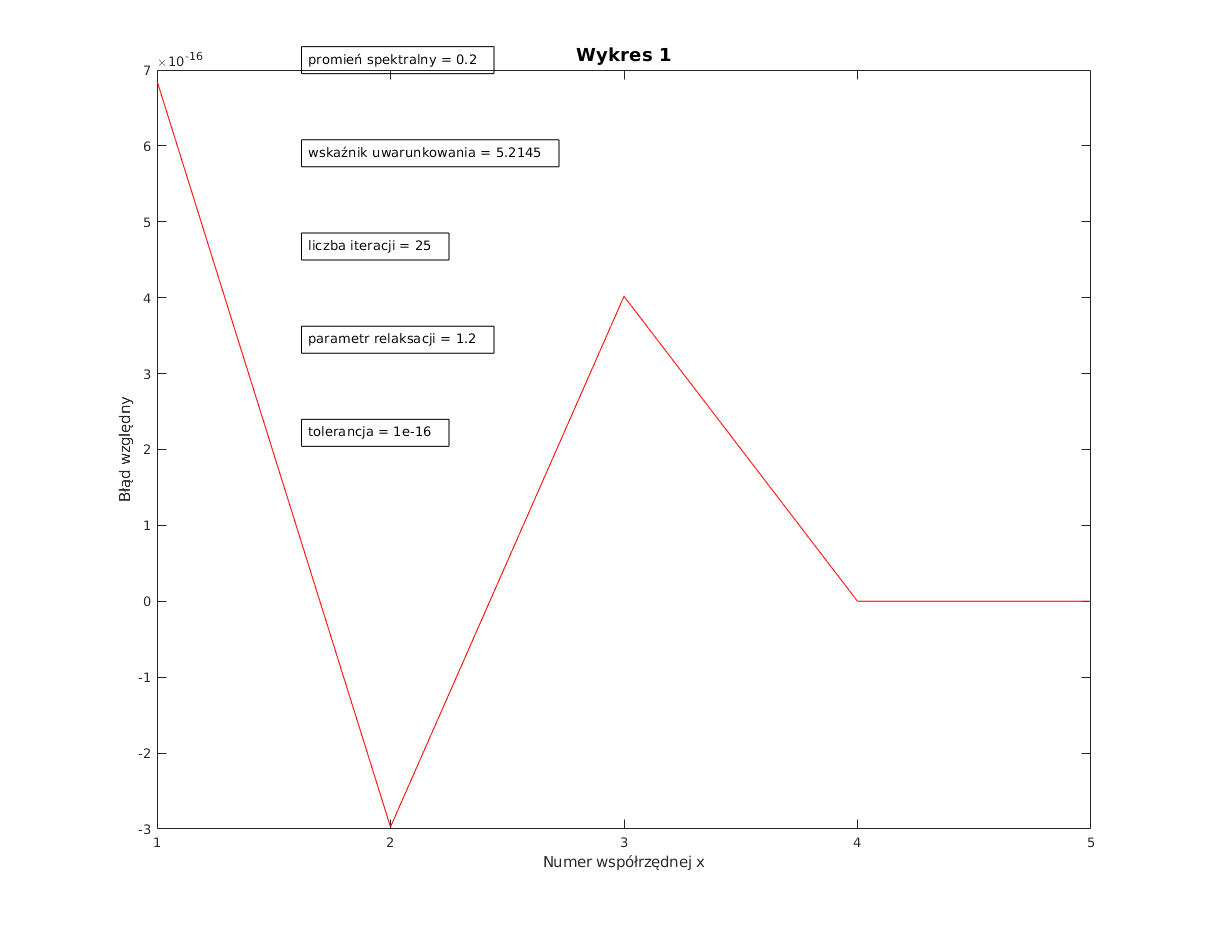
\includegraphics[width = 12cm]{wykres1.png}
    \caption{Wykres przedstawia błąd względny dla kolejnych współrzędnych rozwiązania. Promień spektralny jest mały, więc metoda zbiega szybko. Widać to też po tym, że potrzebne było jedynie 25 iteracji, żeby poradzić sobie z tolerancją $10^{-16}$.}
\end{figure}

\subsection{Przykład 2}
\vskip3ex
\begin{equation}
    A = \begin{pmatrix}
        1 & 0 & 0 & -3 \\
        1 & -1 & 0 & 0 \\
        0 & 0 & 1 & 1 \\
        0 & 0 & -2 & 2 \\
    \end{pmatrix}, 
    b = \begin{pmatrix}
        3 \\
        -1 \\
        -2 \\
        1 \\
    \end{pmatrix}
\end{equation}


\begin{figure}[H]
    \centering
    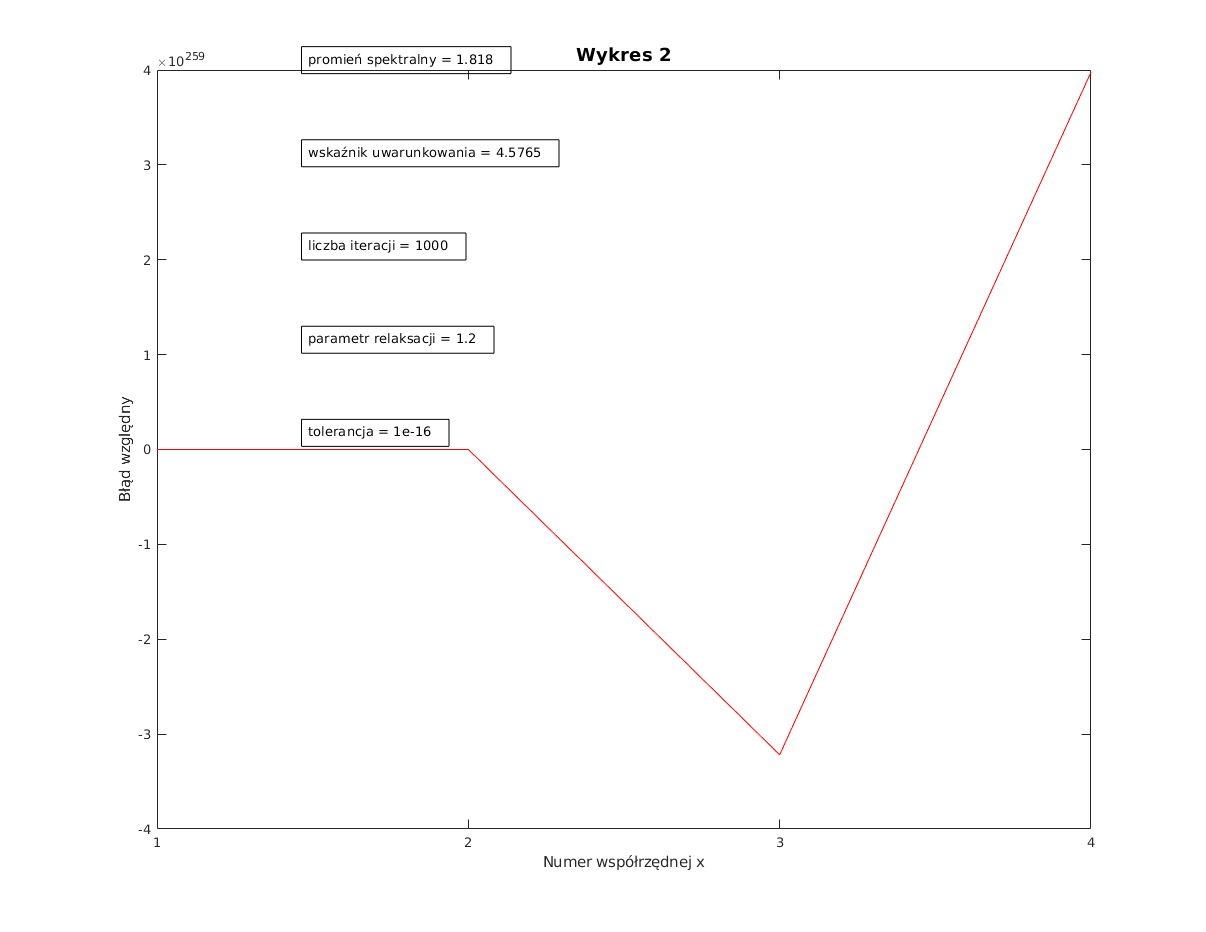
\includegraphics[width = 12cm]{wykres2.png}
    \caption{Wykres przedstawia błąd względny dla kolejnych współrzędnych rozwiązania. Promień spektralny przekracza 1, więc metoda jest rozbieżna. Z tego powodu błąd względny wychodzi ogromny.}
\end{figure}

\subsection{Przykład 3}
\vskip3ex
\begin{equation}
   A = \begin{pmatrix}
        2.04 & -1 & 0 \\
        -1 & 2.04 & -1 \\
        0 & -1 & 2.04\\
    \end{pmatrix}, 
    b = \begin{pmatrix}
        48.8 \\
        0.8 \\
        0.8 \\
    \end{pmatrix}
\end{equation}

\begin{figure}[H]
    \centering
    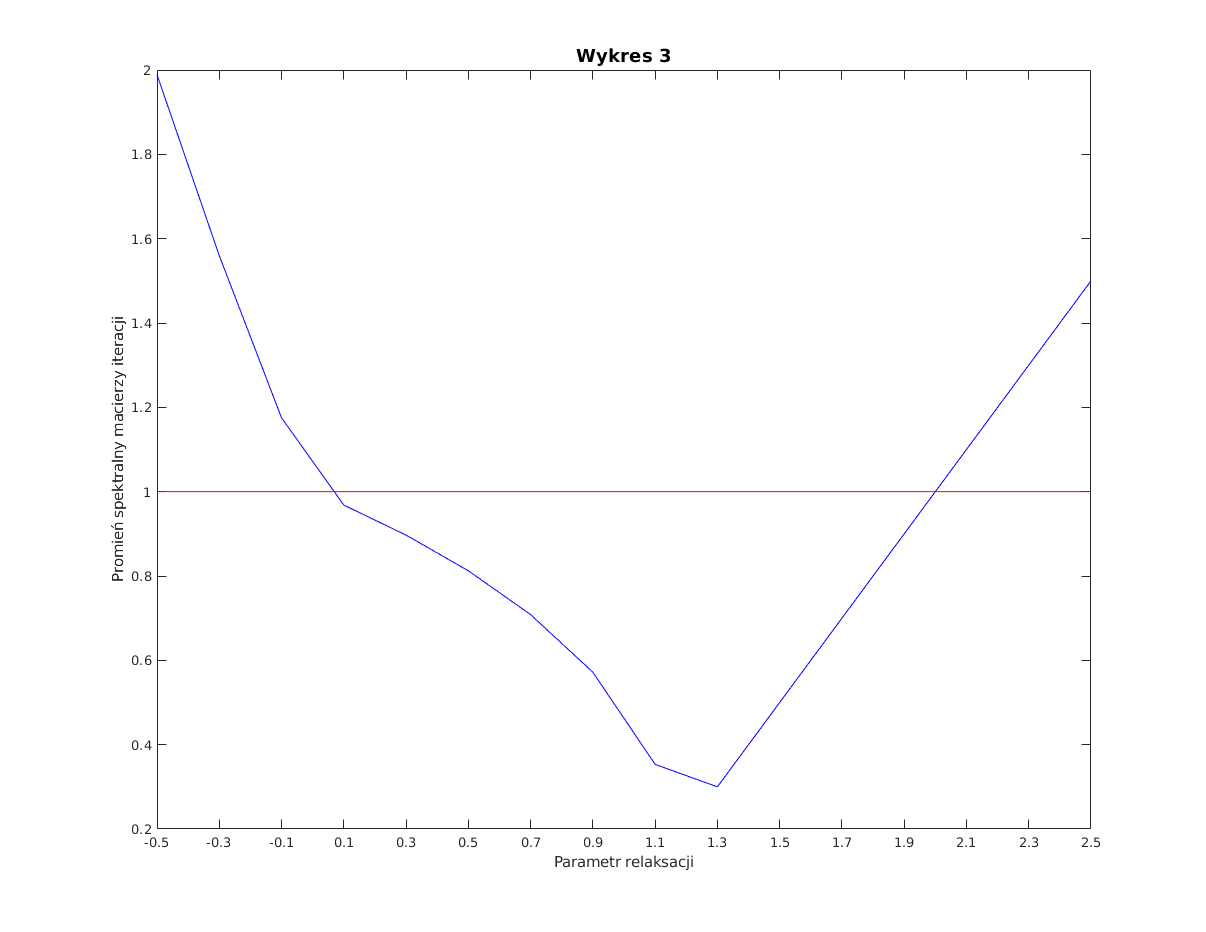
\includegraphics[width = 15cm]{wykres3.png}
    \caption{Wykres przedstawia zależność między parametrem relaksacji a promieniem spektralnym macierzy iteracji. Widać, że promień spektralny jest mniejszy od 1, a więc metoda jest zbieżna, dla $\omega \in (0,2)$. Zbiega natomiast najszybciej dla parametru relaksacji w okolicach $1.3$.}
\end{figure}

\subsection{Przykład 4}
\vskip3ex
\begin{equation}
   A = \begin{pmatrix}
        0 & -1 & -1 \\
        3 & 3 & 3 \\
        -1 & -1 & 0\\
    \end{pmatrix}, 
    b = \begin{pmatrix}
        -1 \\
        7 \\
        7 \\
    \end{pmatrix}
\end{equation}

\begin{figure}[H]
    \centering
    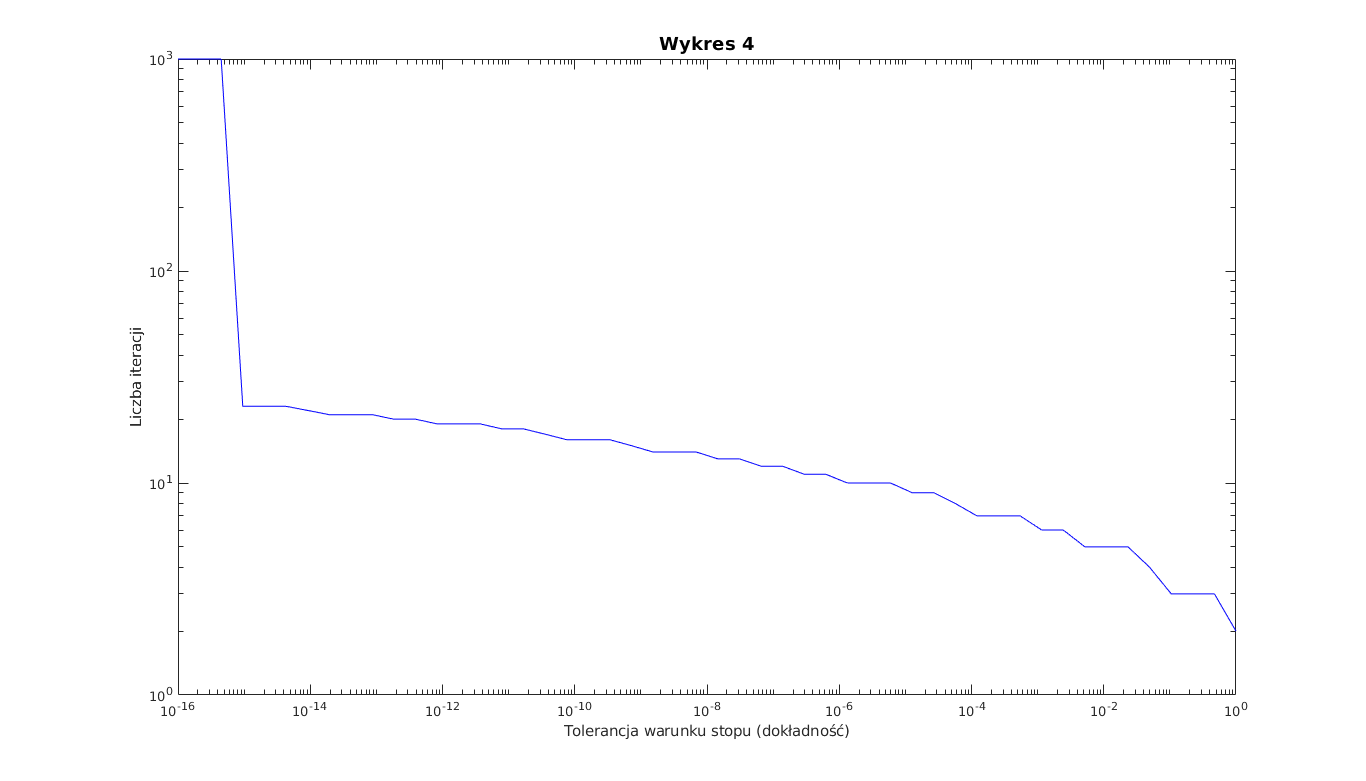
\includegraphics[width = 15cm]{wykres4.png}
    \caption{Wykres przedstawia zależność między tolerancją warunku stopu (dokładnością) a liczbą iteracji. Widać, że im mniejsza tolerancja jest wymagana, tym więcej iteracji potrzeba, aby uzyskać wynik z tą tolerancją. W pewnym momencie również (dla $d\approx 10^{-15.5}$) liczba iteracji przekracza maksymalną liczbę iteracji równą 1000.}
\end{figure}

\subsection{Przykład 5}
\vskip3ex
\begin{equation}
   A = \begin{pmatrix}
        6 & 0 & 0 & 0 & 0 & 0 & 0 \\
        1 & 4 & 1 & 0 & 0 & 0 & 0 \\
        0 & 1 & 4 & 1 & 0 & 0 & 0 \\
        0 & 0 & 1 & 4 & 1 & 0 & 0 \\
        0 & 0 & 0 & 1 & 4 & 1 & 0 \\
        0 & 0 & 0 & 0 & 1 & 4 & 1 \\
        0 & 0 & 0 & 0 & 0 & 0 & 6 \\
    \end{pmatrix}, 
    b = \begin{pmatrix}
        0 \\
        1 \\
        2 \\
        -6 \\
        2 \\
        1 \\
        0 \\
    \end{pmatrix}
\end{equation}

\begin{figure}[H]
    \centering
    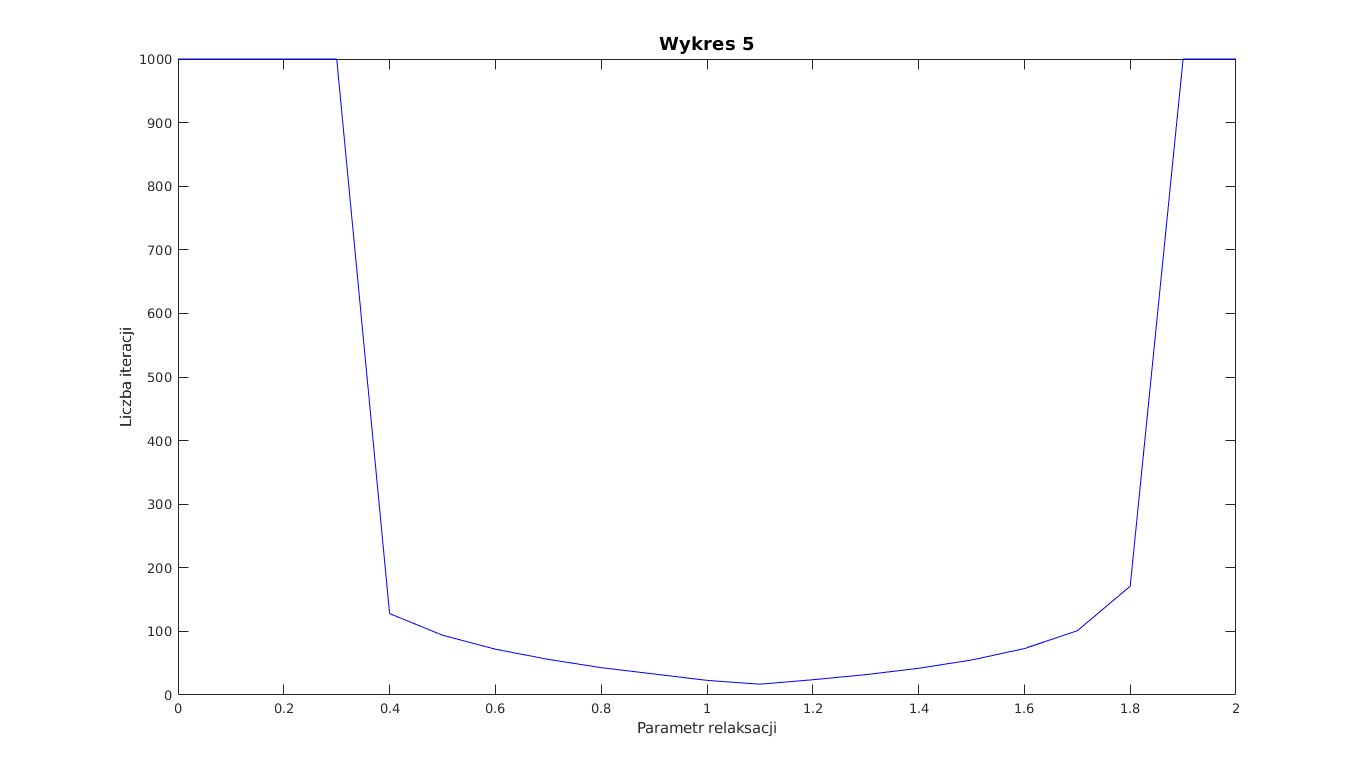
\includegraphics[width = 15cm]{wykres5.png}
    \caption{Wykres przedstawia zależność między parametrem relaksacji a potrzebną liczbą iteracji do uzyskania rozwiązania z daną stałą tolerancją ($d = 10^{-15}$). Wykres przypomina parabolę. Liczba iteracji robi się bardzo duża dla $\omega \in (-\infty,0.4)\cup(1.8,\infty)$.Najmniej iteracji potrzeba dla $\omega \approx 1.1$.}
\end{figure}

\subsection{Przykład 6}
\vskip3ex
\begin{equation}
   A = \begin{pmatrix}
        0 & 0 & 0 & 0 & 0 \\
        0 & 0 & 0 & 0 & 0 \\
        0 & 0 & 0 & 0 & 0 \\
        0 & 0 & 0 & 0 & 0 \\
        0 & 0 & 0 & 0 & 0 \\
    \end{pmatrix}, 
    b = \begin{pmatrix}
        1 \\
        2 \\
        3 \\
        4 \\
        5 \\
    \end{pmatrix}
\end{equation}

\begin{figure}[H]
    \centering
    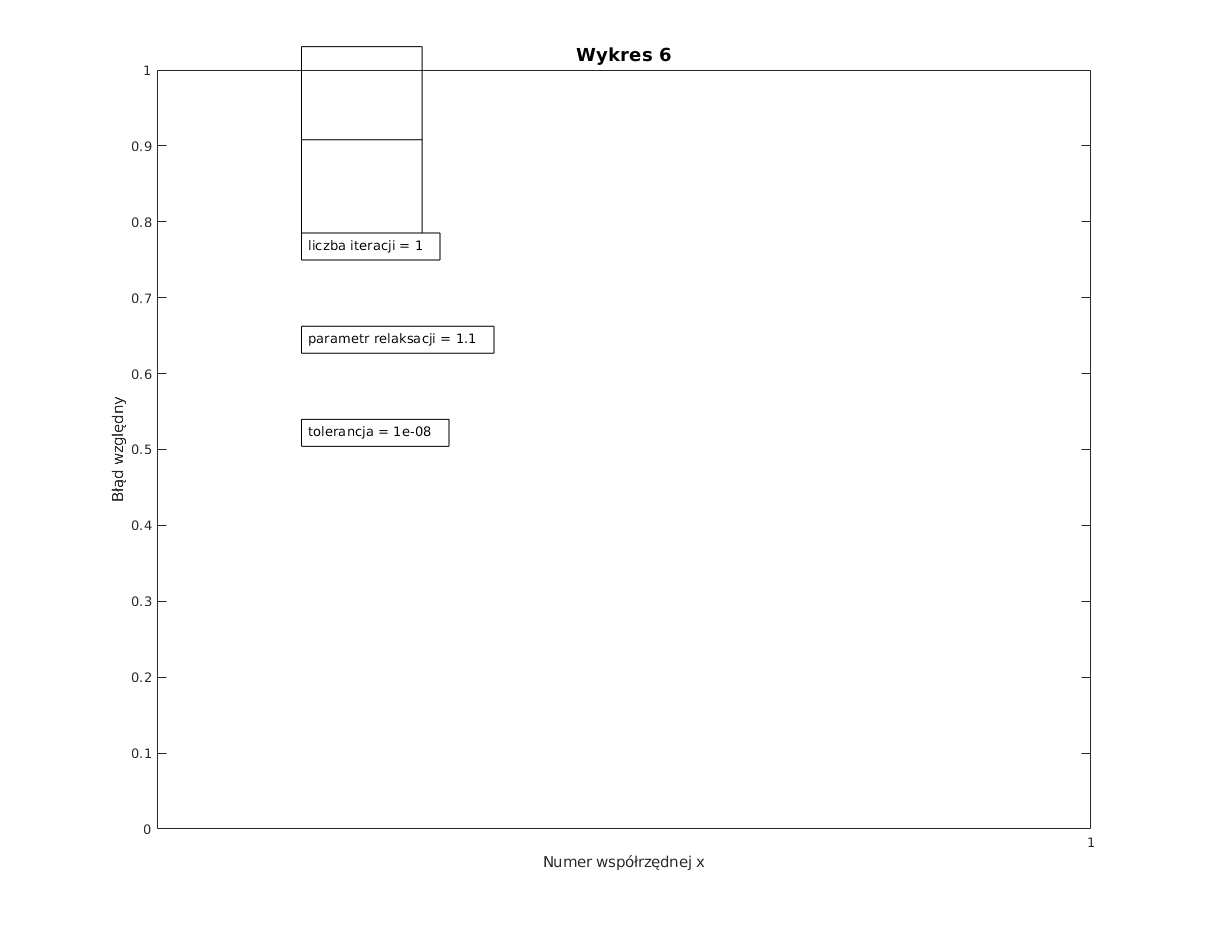
\includegraphics[width = 15cm]{wykres6.png}
    \caption{Co się dzieje w przypadku układu sprzecznego? Program kończy pracę po 1 iteracji. Zwracany jest wektor $(NaN,NaN,NaN,NaN,Inf)^T$}
\end{figure}

\bigskip



\section{Analiza wynik\'ow}

\begin{table}[H]
\caption{\footnotesize Wyniki dla przykładu 1} %\vskip1ex
\renewcommand{\arraystretch}{1.1}
\centering\begin{tabular}{|c|c|c|c|}
\hline L.p. & wartość & wartość & błąd\\
 & dokładna & przybliżona & względny\\
\hline 1 & 0.0506 & 0.0506 & $0.6856e\!-\!15$\\
\hline 2 & 0.1867 & 0.1867 & $-0.2973e\!-\!15$\\
\hline 3 & 0.2763 & 0.2763 & $0.4018e\!-\!15$\\
\hline 4 & 0.3462 & 0.3462 & 0\\
\hline 5 & 0.4017 & 0.4017 & 0\\
\end{tabular}
\end{table}

\begin{table}[H]
\caption{\footnotesize Wyniki dla przykładu 2} %\vskip1ex
\renewcommand{\arraystretch}{1.1}
\centering\begin{tabular}{|c|c|c|c|c|}
\hline L.p. & wartość & wartość & błąd\\
 & dokładna & przybliżona & względny\\
\hline 1 & 3.0000 & 0 & 0\\
\hline 2 & 4.0000 & 0 & 0\\
\hline 3 & -1.2500 & $4.0221e\!+\!259$ & $-3.2176e\!+\!259$\\
\hline 4 & -0.7500 & $-2.9830e\!+\!259$ & $3.9773e\!+\!259$\\
\end{tabular}
\end{table}

\begin{table}[H]
\caption{\footnotesize Wyniki dla przykładu 3} %\vskip1ex
\renewcommand{\arraystretch}{1.1}
\centering\begin{tabular}{|c|c|c|c|}
\hline L.p. & parametr & promień\\
 & relaksacji & spektralny\\
\hline 1 & -0.5000 & 1.9888\\
\hline 2 & -0.3000 & 1.5597\\
\hline 3 & -0.1000 & 1.1752\\
\hline 4 & -0.1000 & 0.9682\\
\hline 5 & -0.2000 & 0.8970\\
\hline 6 & -0.5000 & 0.8124\\
\hline 7 & -0.7000 & 0.7084\\
\hline 8 & -0.9000 & 0.5718\\
\hline 9 & 1.1000 & 0.3532\\
\hline 10 & 1.3000 & 0.3000\\
\hline 11 & 1.5000 & 0.5000\\
\hline 12 & 1.7000 & 0.7000\\
\hline 13 & 1.9000 & 0.9000\\
\hline 14 & 2.1000 & 1.1000\\
\hline 15 & 2.3000 & 1.3000\\
\hline 16 & 2.5000 & 1.5000\\
\end{tabular}
\end{table}

\begin{table}[H]
\caption{\footnotesize Wyniki dla przykładu 4} %\vskip1ex
\renewcommand{\arraystretch}{1.1}
\centering\begin{tabular}{|c|c|c|c|}
\hline L.p. & tolerancja & liczba\\
 & (dokładność) & iteracji\\
\hline 1 & 1 & 2\\
\hline 2 & $10^{-1}$ & 3\\
\hline 3 & $10^{-2}$ & 5\\
\hline 4 & $10^{-3}$ & 7\\
\hline 5 & $10^{-4}$ & 8\\
\hline 6 & $10^{-5}$ & 9\\
\hline 7 & $10^{-6}$ & 11\\
\hline 8 & $10^{-7}$ & 12\\
\hline 9 & $10^{-8}$ & 14\\
\hline 10 & $10^{-9}$ & 15\\
\hline 11 & $10^{-10}$ & 16\\
\hline 12 & $10^{-11}$ & 18\\
\hline 13 & $10^{-12}$ & 19\\
\hline 14 & $10^{-13}$ & 21\\
\hline 15 & $10^{-14}$ & 22\\
\hline 16 & $10^{-15}$ & 23\\
\hline 17 & $10^{-16}$ & 1000\\
\end{tabular}
\end{table}

\begin{table}[H]
\caption{\footnotesize Wyniki dla przykładu 5} %\vskip1ex
\renewcommand{\arraystretch}{1.1}
\centering\begin{tabular}{|c|c|c|c|}
\hline L.p. & parametr & liczba\\
 & relaksacji & iteracji\\
\hline 1 & 0 & 1000\\
\hline 2 & 0.1000 & 1000\\
\hline 3 & 0.2000 & 1000\\
\hline 4 & 0.3000 & 1000\\
\hline 5 & 0.4000 & 128\\
\hline 6 & 0.5000 & 94\\
\hline 7 & 0.6000 & 72\\
\hline 8 & 0.7000 & 56\\
\hline 9 & 0.8000 & 43\\
\hline 10 & 0.9000 & 33\\
\hline 11 & 1.0000 & 23\\
\hline 12 & 1.1000 & 17\\
\hline 13 & 1.2000 & 24\\
\hline 14 & 1.3000 & 32\\
\hline 15 & 1.4000 & 42\\
\hline 16 & 1.5000 & 55\\
\hline 17 & 1.6000 & 73\\
\hline 18 & 1.7000 & 101\\
\hline 19 & 1.8000 & 171\\
\hline 20 & 1.9000 & 1000\\
\hline 21 & 2.0000 & 1000\\

\end{tabular}
\end{table}

\begin{table}[H]
\caption{\footnotesize Wyniki dla przykładu 6} %\vskip1ex
\renewcommand{\arraystretch}{1.1}
\centering\begin{tabular}{|c|c|c|c|}
\hline L.p. & wartość & wartość & błąd\\
 & dokładna & przybliżona & względny\\
\hline 1 & NaN & NaN & NaN\\
\hline 2 & NaN & NaN & NaN\\
\hline 3 & NaN & NaN & NaN\\
\hline 4 & NaN & NaN & NaN\\
\hline 5 & NaN & Inf & NaN\\
\end{tabular}
\end{table}

Na podstawie wyników można zauważyć kilka obserwacji:
\begin{itemize}
    \item gdy metoda zbiega szybko, mało iteracji jest potrzebnych do uzyskania nawet bardzo dokładnych wyników,
    \item gdy metoda jest rozbieżna, błąd względny wychodzi bardzo duży,
    \item metoda jest rozbieżna, gdy $\omega \notin (0,2)$,
    \item metoda zbiega najszybciej dla $\omega \approx 1.3$,
    \item przy zmniejszaniu tolerancji zwiększa się liczba potrzebnych iteracji,
    \item w przypadku $d = 10^{-15}$ liczba iteracji przekracza 100 dla $\omega \in (-\infty,0.4)\cup(1.8,\infty)$,
    \item najmniej iteracji potrzeba dla $\omega \approx 1.1$.
\end{itemize}

\end{document}